\documentclass{beamer}
\usetheme{Antibes}

\usepackage{graphicx} % Required for inserting images
\usepackage[brazilian]{babel}
\usepackage[sorting=none]{biblatex}
\addbibresource{referencias.bib}
\DeclareBibliographyCategory{cited} % Separa referências citadas das não citadas
\AtEveryCitekey{\addtocategory{cited}{\thefield{entrykey}}}
\usepackage{amsmath}
\usepackage{algorithm,algorithmic}
\usepackage{tikz}
\usetikzlibrary{arrows.meta, calc, quotes, tikzmark}

% Faz a fonte da matemática ficar bonita
\renewcommand\mathfamilydefault{\rmdefault} 
\setlength{\columnsep}{2cm}

% Separa as seções
\AtBeginSubsection[]{
  \begin{frame}
  \vfill
  \centering
  \begin{beamercolorbox}[sep=8pt,center,shadow=true,rounded=true]{title}
    \usebeamerfont{title}\insertsectionhead\par%
    \vspace{6pt}
    \usebeamerfont{subtitle}{\small \textbf{\insertsubsectionhead}}
  \end{beamercolorbox}
  \vfill
  \end{frame}
}

\title{Otimização aplicado à logística}
%\author{Alan Peterson, Erick Manjarra, Felipe Gomes, Felipe Kuang, Fernando Dias, Lucas Tiné}
% Novo arranjo de nomes proposto por Felipe Kuang
\author[Alan Peterson, Erick Manjarra, Felipe Gomes, Felipe Kuang, Fernando Dias, Lucas Tiné]{%
  \texorpdfstring{%
    \begin{columns}
      \column{.3\linewidth}
      \centering
      Alan Peterson
      \column{.3\linewidth}
      \centering
      Felipe Kuang 
    \end{columns}
    \vspace{1pt}
    \begin{columns}
      \column{.3\linewidth}
      \centering
      Erick Manjarra
      \column{.3\linewidth}
      \centering
      Fernando Dias 
    \end{columns}
    \vspace{1pt}
    \begin{columns}
      \column{.3\linewidth}
      \centering
      Felipe Gomes
      \column{.3\linewidth}
      \centering
      Lucas Tiné
    \end{columns}
 }
 {Alan Peterson, Erick Manjarra, Felipe Gomes, Felipe Kuang, Fernando Dias, Lucas Tiné}
}
\date{13 de junho de 2023}

% "Pula uma linha" depois dos bullets (gosto dessa formatação)
\newenvironment{outeritemize}{\begin{itemize}}{\end{itemize}\vspace{12pt}}

% Remove barra de navegação e coloca número de slides
\setbeamertemplate{navigation symbols}{}
\setbeamertemplate{footline}[frame number]


\begin{document}

\begin{frame}
    \maketitle
\end{frame}

\begin{frame}{Agenda}
    \tableofcontents
\end{frame}



\begin{frame}{\textit{Disclaimer}}
    Base do material: Curso \texttt{CPE728} da COPPE (Prof. Rodrigo) \cite{CPE728CursoOtimizacaoAplicadaasRedesComputadoresYouTube_www.youtube.com}
    \begin{columns}
        \column{0.35\textwidth}
        \begin{figure}
            \centering
            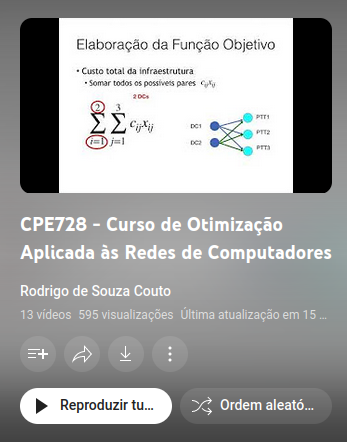
\includegraphics[width=\textwidth]{assets/Introducao/PlaylistRodrigoThumbnail.png}
        \end{figure}
        \column{0.65\textwidth}
        \begin{figure}
            \centering
            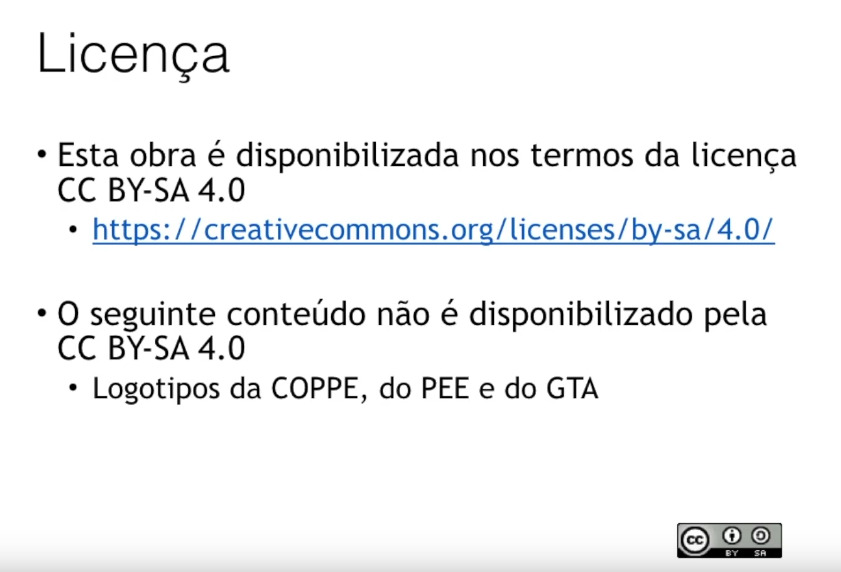
\includegraphics[width=\textwidth]{assets/Introducao/PlaylistRodrigoLicenca.png}
        \end{figure}
    \end{columns}
    \vspace{12pt}
    Essa apresentação é portanto licenciada \texttt{(CC BY-SA 4.0)}
\end{frame}

\section{Introdução}

\subsection*{Conceitos de otimização}

\begin{frame}{Otimização}
    \begin{block}{Definição}
        Otimização é a busca das variáveis que maximizam ou minimizam uma função objetivo
    \end{block}
    \vspace{12pt}
    Método de resolução
    \begin{enumerate}
       \item Variáveis de decisão: $\vec{x}=\begin{bmatrix} x_1 & x_2 & \dots & x_n\end{bmatrix}$
       \item Função objetivo: $\min f(\vec{x})$ ou $\max f(\vec{x})$
       \item Restrições $\vec{c}(\vec{x})$
       \begin{itemize}
           \item Igualdades $c_i(\vec{x})=0\;\forall\;i\in\mathcal{E}$
           \item Desigualdades $c_i(\vec{x})\leq0\;\forall\;i\in\mathcal{I}$
       \end{itemize}
    \end{enumerate}
\end{frame}

\note{Apresentar a nomeclatura e explicar quais são os componentes. \\ Deixar claro que a mesma ordem de aparição dos componentes é a ordem do método de modelagem de um problema de otimização.}

\begin{frame}{Resolução de um problema de otimização}{Caracterização}
Definições do problema
\begin{outeritemize}    
    \item Conjuntos das variáveis: $\mathbb{Z}$, $\mathbb{R}$, etc...
    \item Tipo de modelo: Linear Vs. Não-linear
    \item Conjunto viável: Restrições Vs. Sem restrições
\end{outeritemize}
Tipo de solução
\begin{outeritemize}    
    \item Solução global Vs. local
\end{outeritemize}
Objetivo de modelagem: \textit{Programação linear}
\end{frame}

\note{Justificar a necessidade de linearização devido à presença de inúmeros algoritmos e possibilidade de chegar no resultado ótimo (solução global). \\ \vspace{12pt} Curiosidade: Falar que ``programação'' era o nome dado na década de 40 antes da associação do nome com programas de computador.}

\subsection*{Ambientação em logística}

\begin{frame}{Introdução à logística}
    \begin{block}{Definição}
        \textit{``Logística está preocupada com a organização, movimento e armazenamento de materiais e pessoas.''}
        \begin{flushright}
            Prefácio de \cite{ghiani.etal_2004}, tradução livre.
        \end{flushright}
    \end{block}
    \vspace{12pt}
    Elementos de logística
    \begin{itemize}
        \item Planejamento do sistema logístico
        \item Acomodação das rotas de transporte
        \item Gerenciamento de estoque
    \end{itemize}
    
\end{frame}

\note{
Esse é um exemplo de nota, que podem ser compiladas junto ou separado do slide (o trabalho final não acompanha essas anotações). 
}

\note{
Listagem de conceitos a serem apresentados em cada problema
\begin{itemize}
    \item Melhor localização $\to$ Introdução à notação e conceitos
    \item Linearização de variáveis binárias
    \item Linearização de variáveis lógicas
    \item Discussão otimização Vs. algoritmo exato
    \item Problema de fluxo máximo $\to$ ???
    \item ??? $\to$ ???
\end{itemize}
}

\note{
Listagem de contextualização de cada problema
\begin{itemize}
    \item Melhor localização $\to$ Posicionamento de um centro de distribuição
    \item P-centros $\to$ Posicionamento de $p$-centros de distribuição(?)
    \item 
\end{itemize}

}

\begin{frame}{Ferramentas utilizadas}
    Soluções prontas
    \begin{itemize}
        \item \textit{Warehouse Management System }(WMS)
        \item \textit{Transport Management System} (TMS)
        \item \textit{Manufacturing Resource Planning} (MRS)
    \end{itemize}
    \textbf{Problema}: Pagas/software sob demanda
    \vspace{12pt}
    
    Soluções específicas
    \begin{itemize}
        \item Resolvedor (\textit{Solver}): PuLP (Python3)
    \end{itemize}
    \textbf{Problema}: Como modelar?
\end{frame}

\begin{frame}{Problemas de logística}{Exemplos de aplicação}
    Centros de distribuição
    \begin{outeritemize}
        \item Planejamento de localização
        \item Escoamento de produtos
    \end{outeritemize}
    Transporte
    \begin{outeritemize}
        \item Custos de locomoção
        \item Planejamento de rotas
    \end{outeritemize}
    \vspace{12pt}
    Sempre quando o problema é
    \begin{center}
        \textbf{Minimizar} custos ou \textbf{maximizar} ganhos
    \end{center}
\end{frame}

\section{Problemas de otimização}

% Fernando Dias
\subsection{Melhor distribuição}

\begin{frame}{Melhor distribuição}{Apresentação do problema}
    \begin{figure}
    \centering
    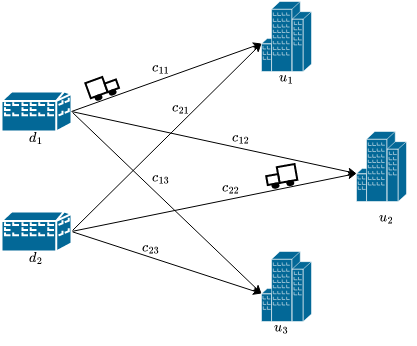
\includegraphics[width=0.6\textwidth]{assets/MelhorLocalizacao/ExemploMelhorLocalizacao.drawio.png}
    \end{figure}
\end{frame}

\begin{frame}{Modelagem do problema}{Definição das variáveis}
    Notação de conjunto
    \begin{outeritemize}
        \item $\mathcal{U}$ clientes
        \item $D$ Centros de Distribuição (CD)
    \end{outeritemize}
    Variável de demanda $x_{ij}$
    \begin{outeritemize}
        \item Quantidade de produto do centro $i$ para o cliente $j$
        \item $x_{ij}\in \mathbb{Z}^{+}_{0}$
    \end{outeritemize}
    Custos associados
    \begin{itemize}
        \item Custos por volume de produto $c_{ij}\propto x_{ij}$
        \item Custos fixos por ``ativação'' do CD $f_i$
    \end{itemize}
\end{frame}

\begin{frame}{Modelagem do problema}{Função objetivo}
    Objetivo
    \begin{outeritemize}
        \item Minimizar o custo \textbf{global}
        \item Somatório de custo dos $\mathcal{D}$ C.D.s
    \end{outeritemize}
    \begin{equation*}
       \min f(\vec{x})= \sum_{i\in\mathcal{D}}\sum_{j\in\mathcal{U}}c_{ij}x_{ij} + \sum_{i\in\mathcal{D}}f_iy_i
    \end{equation*}
    \vspace{12pt}
    
    Onde temos:
    \begin{itemize}
        \item $c_{ij}\to$ Custo de envio do CD $i$ pro cliente $j$
        \item $f_i\to$ Custo fixo de transporte do CD $i$
        \item $y_i\to$ Variável \textit{condicional} que diz se o CD $i$ foi ativado
    \end{itemize} 

    \vspace{12pt}
    Obs: $i\in\mathcal{D}$ ``Todos os centros em $\mathcal{D}$''
\end{frame}

\begin{frame}{Modelagem do problema}{Restrições}
    Cada cliente tem uma demanda $d_i$
    \begin{equation*}
        \sum_{i\in\mathcal{D}}x_{ij}=d_i \;\forall\;j\in\mathcal{U}
    \end{equation*}
    Cada centro só pode atender até uma demanda máxima $b_j$     
    \begin{equation*}
        \sum_{j\in\mathcal{U}} x_{ij}<b_j \;\forall\; i\in\mathcal{D}
    \end{equation*}
\end{frame}

\begin{frame}{Modelagem do problema}{Variável auxiliar}
    Representação de uma variável condicional
    \begin{align*}
        y_i = & \begin{cases}
            1,\;\text{se} \sum_{j\in\mathcal{U}}x_{ij}>0\\
            0,\;\text{senão}
        \end{cases}
    \end{align*}
    \textbf{Problema}: Não é linear!\\
    \vspace{12pt}
    \textit{Solução}: Linearização da variável
    \begin{align*}
        My_i\ge\sum_{j\in\mathcal{U}}x_{ij}\;\forall i \in \mathcal{D} \Longrightarrow  My_i - \sum_{j\in\mathcal{U}}x_{ij}\ge0\;\forall i \in \mathcal{D}
    \end{align*}
    Onde $M$ é um número muito grande e $y_i\in\{0,1\}$
\end{frame}


\begin{frame}{Modelagem do problema}{Resultado final}
    Para $\mathcal{D}$ centros de distribuição e $\mathcal{U}$ clientes, queremos:
    \begin{equation*}
        f(\vec{x})=\min\sum_{i\in\mathcal{D}}\sum_{j\in\mathcal{U}}c_{ij}x_{ij} + \sum_{i\in\mathcal{D}}f_iy_i
    \end{equation*}

    Onde,
    \begin{equation*}
        \sum_{i\in\mathcal{D}}x_{ij}=d_i \;\forall\;j\in\mathcal{U}
    \end{equation*}
    \begin{equation*}
        \sum_{j\in\mathcal{U}} x_{ij}<b_j \;\forall\; i\in\mathcal{D}
    \end{equation*}
    \begin{equation*}
        My_i - \sum_{j\in\mathcal{U}}x_{ij}\ge0\;\forall i \in \mathcal{D}    
    \end{equation*}
    E finalmente, $x_{ij}\in\mathbb{Z}^{+}_{0}$, $y_i\in\{0,1\}$ e $c_{ij}\in\mathbb{R}$.
\end{frame}


\begin{frame}{Resolução do problema}{Uso das ferramentas}
    Implementação no PuLP
    \begin{outeritemize}
        \item Exemplo na documentação: \textit{A transportation problem} \cite{PuLP_coin}
    \end{outeritemize}
    Variações no caso
    \begin{outeritemize}
        \item Excedente de produção
        \item Perdas pra competidores
    \end{outeritemize}
    Programação dinâmica
    \begin{itemize}
        \item Variação dos custos ao longo dos meses
        \item Integração com ferramentas
        \item Adição e remoção de clientes 
    \end{itemize}
\end{frame}

% Lucas Tiné
\subsection{P-centros}

\begin{frame}{Apresentação}

\begin{figure}
    \centering
    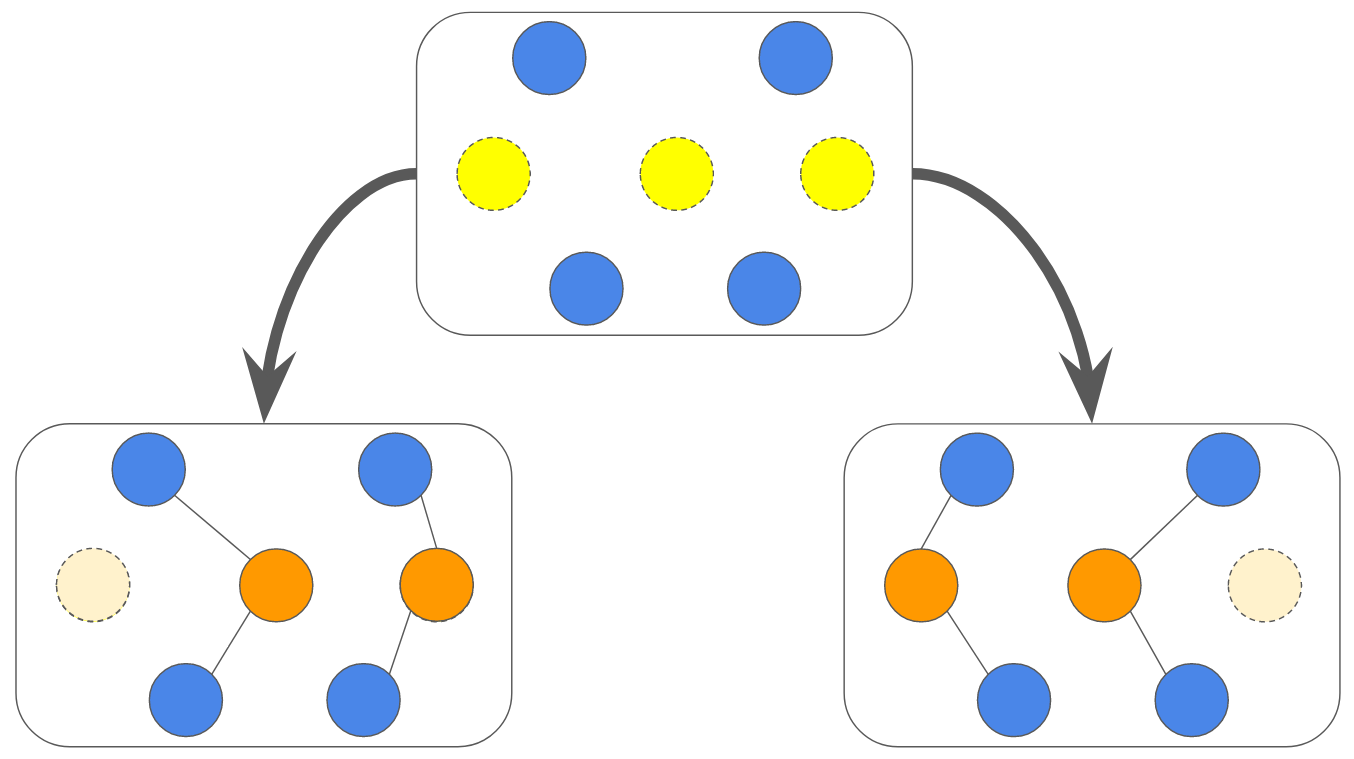
\includegraphics[width=0.7\textwidth]{assets/PCentros/p-centros.png}
    \end{figure}

    \begin{itemize}
        \item P-centros atenderão N consumidores, e podem ser instalados em M locais de instalação.
        \item Objetivo: minimização do pior caso, ou menor custo máximo ("minimax")
    \end{itemize}
\end{frame}

\note{Diferença principal do problema anterior: Quantidade de centros de distribuição \textbf{a definir}. \\ \vspace{12pt} Apresente o conceito de custo fixo (o que implica variáveis de decisão). \\ \vspace{12pt} 
}

\begin{frame}{Formulação do problema}{Rascunho}

Temos os seguintes parâmetros:
\begin{outeritemize}
    \item Precisa-se abrir $\mathcal{P}$ instalações para atender $\mathcal{U}$ consumidores
    \item Cada instalação $i$ atende o consumidor $j$ com custo $c_{ij}$.
\end{outeritemize}

E as variáveis de decisão:
\begin{outeritemize}
    \item $x_{ij}$ indica se a instalação $i$ atenderá o consumidor $j$
    \item $y_{i}$ se no local $i$ haverá uma instalação (variável binária).
    \item Dentre $\mathcal{F}$ locais possíveis, posso instalar $p$ centros de distribuição (fornecedores)
    \item $\mathcal{C}$ é a maior custo possível na solução
\end{outeritemize}

\end{frame}

\begin{frame}{Modelagem do problema}{Restrições dos parâmetros}
    
    \begin{enumerate}
        \item Cada consumidor é atendido por apenas uma instalação 
        
        \begin{equation*}
            \sum_{\mathcal{U}} x_{ij} = 1 \;\forall\;j \in\mathcal{U}
        \end{equation*} 
    
        \item Para uma instalação atender um consumidor, ela deve existir

        \begin{equation*}
            x_{ij} - y_i \leq 0 \;\forall\;i \in\mathcal{P} ;j \in \mathcal{U}
        \end{equation*}

        \item Exatamente $p$ instalações no conjunto de locais possíveis
        \begin{equation*}
            \sum_{\mathcal{P}} y_{i} = p 
        \end{equation*} 

    \end{enumerate}
      
\end{frame}

\begin{frame}{Modelagem do problema}{Restrições da função objetivo}
    
    \begin{enumerate}
        \item $\mathcal{C}$ é sempre maior ou igual ao maior custo de suprimento utilizado

        \begin{equation*}
            \sum_{\mathcal{P}} c_{ij} \cdot x_{ij} - \mathcal{C} \leq 0
            \;\forall\;j \in \mathcal{U}
        \end{equation*} 

        \item $x_{ij} = \{0,1\}$, $y_i = \{0,1\}$
    \end{enumerate}
      
\end{frame}

\begin{frame}{Modelo final}
    Objetivo:
    $$\min f(x)= C$$
    Sujeito a:
    $$\sum_{\mathcal{U}} x_{ij} = 1 \;\forall\;j \in\mathcal{U}$$
    $$x_{ij} - y_i \leq 0 \;\forall\;i \in \mathcal{P};  \;\forall\;j \in \mathcal{U}$$
    $$\sum_{\mathcal{P}} y_{i} = p$$ 
    $$\sum_{\mathcal{P}} c_{ij} \cdot x_{ij} - \mathcal{C} \leq 0  \;\forall j \in \mathcal{U}$$
    $$x_{ij} = \{0,1\}, y_i = \{0,1\}$$
\end{frame}

% Felipe Kuang
\subsection{P-dispersão}

\begin{frame}{O problema P-dispersão}
Objetivo
\begin{outeritemize}
    \item Determinar a localização de $p$ facilidades em uma rede\\
\end{outeritemize} 

Caracteristicas
\begin{outeritemize}
    \item A nova instalação deve ser o mais longe possível da outra facilidade mais próxima 
    \item Dispersar para aumentar a área de atuação 
    \item Não há nós de demanda e nem alocação de nós já existentes para outros nós
\end{outeritemize}
\end{frame}

\begin{frame}{Função objetivo}
\[\max f(x)=D\]
\[D \leqslant d_{ij}(1 + M(1 - x_i) + M(1 - x_j)) \quad\forall(i, j)\in{N}\mid{i<j}\]
\[x_i\in\left[0,1\right]\quad\forall{i}\in N\]
\[ \sum_{i=1}^{n} x_i = p \]


Onde\\
\quad{$n$ = número de possíveis facilidades}\\
\quad{$p$ = número de facilidades a instalar}\\
\quad{$N$ = conjunto de nós}\\
\quad{$d_{ij}$ = menor distancia entre os nós \textit{i} e \textit{j}}\\
\quad{$M =$ um número qualquer muito grande} 
\end{frame}

\begin{frame}{Possíveis resultados}
\begin{equation*}
  D\leqslant
    \begin{cases}
      d_{ij}         & \text{se $x_i$ = 1 e $x_j$ = 1}\\
      d_{ij}(1 + M)  & \text{se $x_i$ = 1 ou $x_j$ = 1}\\
      d_{ij}(1 + 2M) & \text{se $x_i$ = 0 e $x_j$ = 0}
    \end{cases}       
\end{equation*}
\begin{itemize}
    \item Apenas os casos onde ambas facilidades estejam abertas irão afetar no valor de $D$
    \item O máximo valor de $D$ será determinado por $d_{ij}$
\end{itemize}
\end{frame}

% \begin{frame}{Características}
% \vspace{0.35cm}
% \qquad Determinação de $D$
% \begin{figure}[3nos]
%     \centering
%     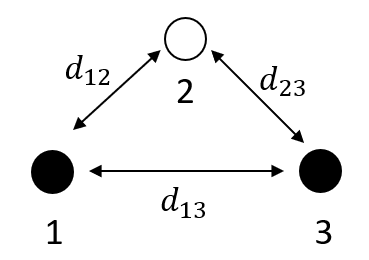
\includegraphics[width=0.3\textwidth]{assets/PDispersao/3 nos.png}
%     \label{fig:3nos}
% \end{figure}
% \begin{figure}[fluxo]
%     \centering
%     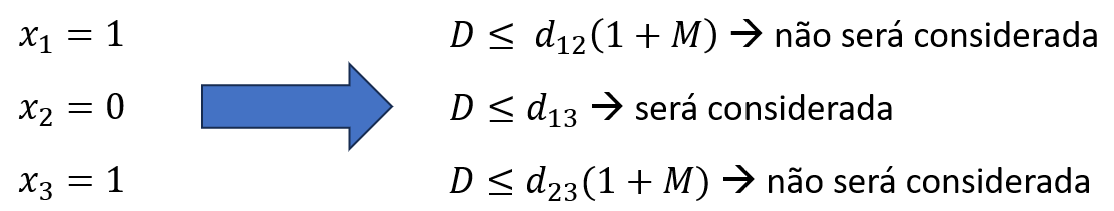
\includegraphics[width=0.9\textwidth]{assets/PDispersao/fluxo condicoes.png}
%     \label{fig:fluxo}
% \end{figure}
% \begin{itemize}
%     \item Portanto, $D = d_{13}$
% \end{itemize} 
% \begin{columns}
% \tikzset{box/.style={inner xsep=0pt}}
% \column{.5\textwidth}
% \begin{itemize}
% \setlength{\itemindent}{3em}
%     \item $X_1 = 1$
%     \item $X_2 = 0$\tikzmark{b}
%     \item $X_3 = 1$
% \end{itemize}
% \column{.5\textwidth}
% \begin{itemize}
% \setlength{\itemindent}{-1em}
%      \item $d_{12}$ não será considerada
%      \item \tikzmark{f}$d_{13}$ será considerada
%      \item $d_{23}$ não será considerada
% \end{itemize}
% \end{columns}

% \begin{tikzpicture}[overlay,remember picture]
%   \draw[very thick, -Stealth]         ($({pic cs:b})+(5ex,0.5ex)$)
%         to [left, sloped, "text"]  ($({pic cs:f})+(-6ex,0.2em)$);
% \end{tikzpicture}
% \end{frame}

% \begin{frame}{Características}
% \qquad Determinação de $D$
% \vspace{0.3cm}
% \begin{figure}[3-nospeso]
%     \centering
%     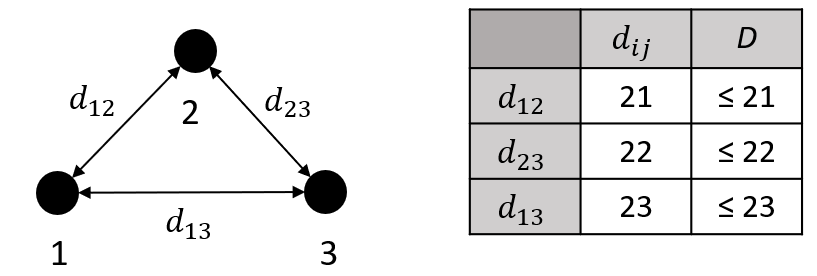
\includegraphics[width=0.6\textwidth]{assets/PDispersao/3 nos com peso.png}
%     \label{fig:3-nospeso}
% \end{figure}
% \begin{itemize}
%     \item O valor de $D$ será determinado pelo menor $d_{ij}$
%     \item No exemplo, $D = 21$ e as outras distâncias devem ser, obrigatoriamente, iguais ou maiores que $D$
% \end{itemize}
% \end{frame}

\begin{frame}{Determinação de D}
% \vspace{0.3cm}
\begin{figure}[4-nos]
    \centering
    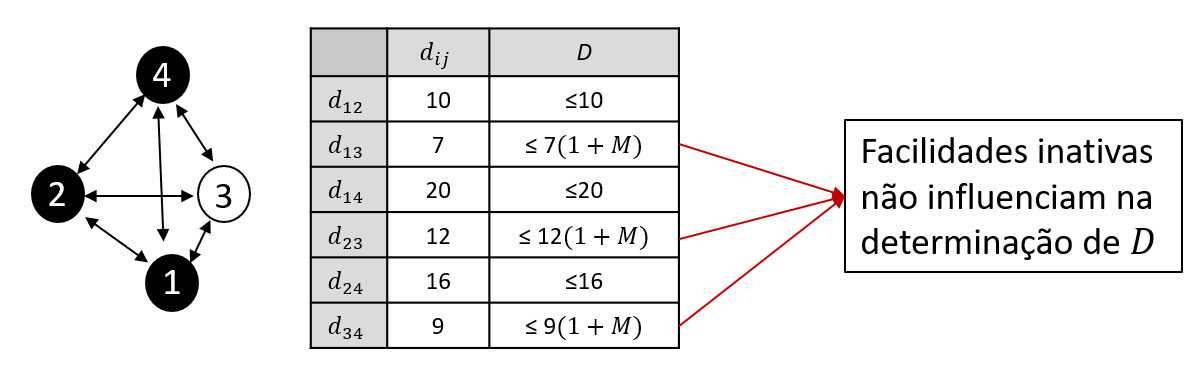
\includegraphics[width=0.95\textwidth]{assets/PDispersao/4 nos.png}
    \label{fig:4-nos}
\end{figure}
\begin{itemize}
    \item O valor de $D$ será determinado pelo menor $d_{ij}$ entre facilidades ativas
    \item Determinado $D$, as outras distâncias devem ser, obrigatoriamente, iguais ou maiores que $D$
\end{itemize}
\end{frame}

% \begin{frame}{Características}
% \vspace{0.2cm}
% \quad Podemos ter mais de uma solução ótima
% \vspace{0.3cm}
% \begin{figure}[2-dispersion]
%     \centering
%     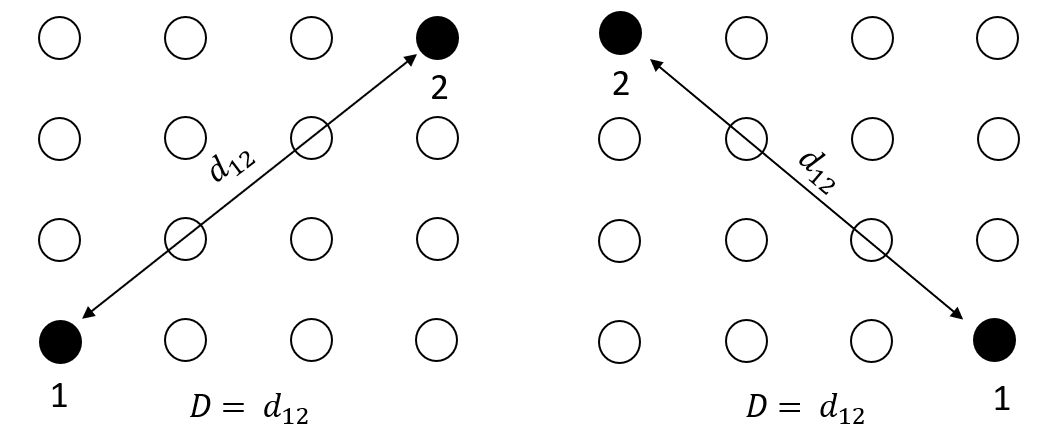
\includegraphics[width=0.8\textwidth]{assets/PDispersao/2-dispersion.png}
%     \caption{Solução para o problema de 2-dispersão}
%     \label{fig:2-dispersion}
% \end{figure}      
% \end{frame}

% Fernando: Mesmo exemplo da anterior, pode descartar
\begin{frame}{Características}
\vspace{0.4cm}
\quad Podemos ter mais de uma solução ótima
\vspace{0cm}
\begin{figure}[3-dispersion]
    \centering
    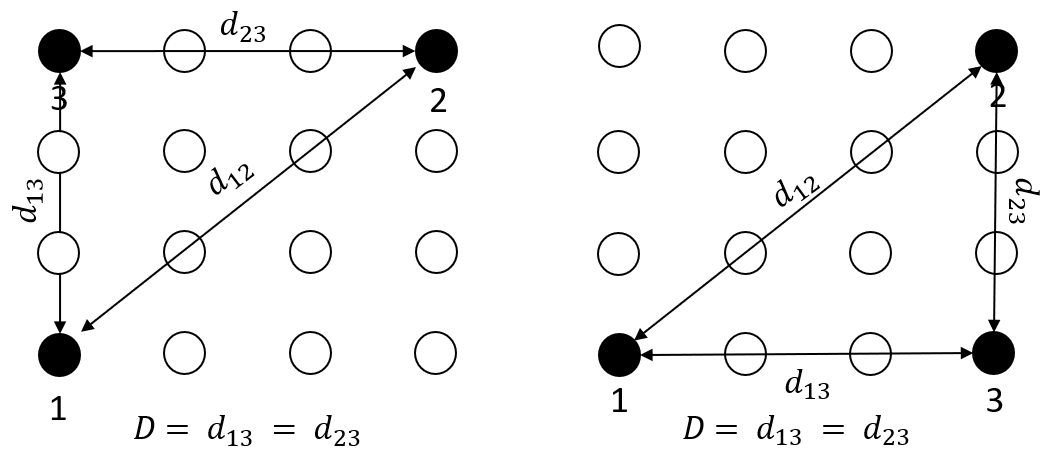
\includegraphics[width=0.85\textwidth]{assets/PDispersao/3-dispersion.png}
    \caption{Solução para o problema de 3-dispersão}
    \label{fig:3-dispersion}
\end{figure}      
\end{frame}

% Fernando: Mesmo exemplo da anterior, pode descartar
% \begin{frame}{Exemplo}
% \begin{figure}[5-dispersion]
%     \centering
%     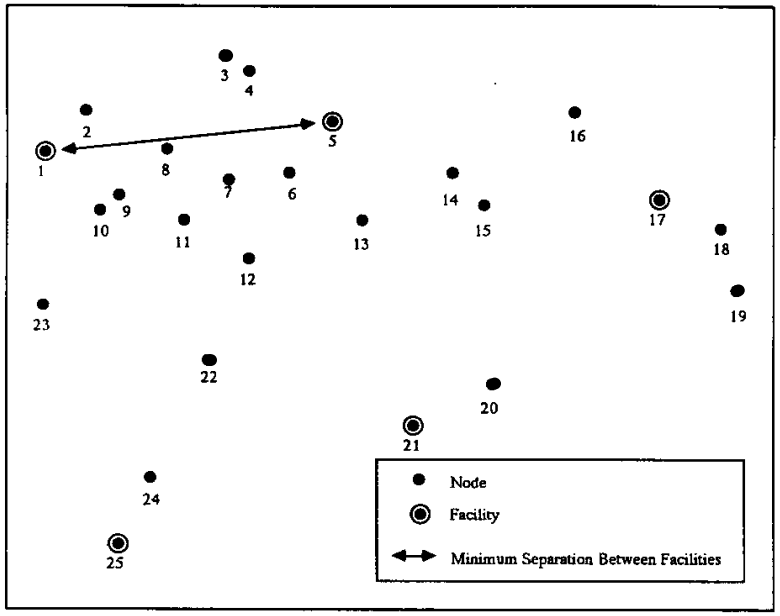
\includegraphics[width=0.65\textwidth]{assets/PDispersao/5-dispersion.png}
%     \caption{Solução para o problema de 5-dispersão}
%     \label{fig:5-dispersion}
% \end{figure}  
% \end{frame}

\begin{frame}{Características}
    \begin{columns} 
    \begin{column}{.5\textwidth}
        \begin{figure}[4-dispersion]
            \centering
            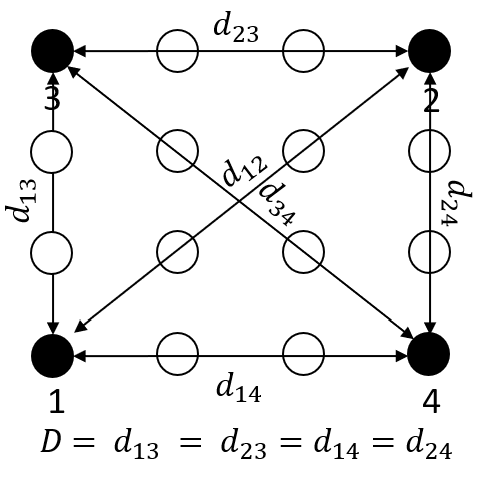
\includegraphics[scale=0.7]{assets/PDispersao/4-dispersion.png}
            \caption{Solução para o problema de 4-dispersão}
            \label{fig:4-dispersion}
        \end{figure}
    \end{column}
    \begin{column}{.5\textwidth}
        \begin{itemize}
            \item O valor de $D$ diminui ou se mantém com o aumento de facilidades
            \item Por exemplo, para $p = 5$, o valor de $D$ será menor
        \end{itemize}
    \end{column}
    
\end{columns}
\end{frame}

% Fernando: Mesmo exemplo da anterior, pode descartar
\begin{frame}{Exemplo}
\begin{figure}[10-dispersion]
    \centering
    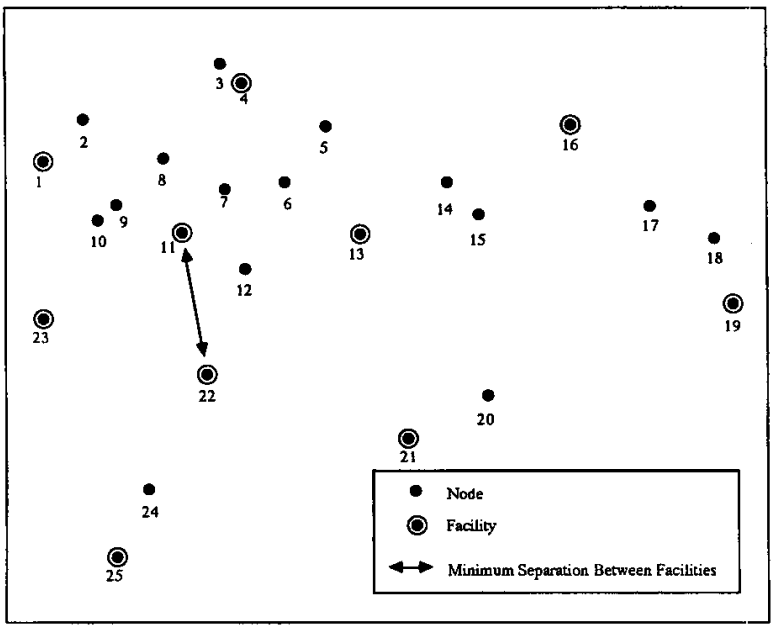
\includegraphics[width=0.65\textwidth]{assets/PDispersao/10-dispersion.png}
    \caption{Solução para o problema de 10-dispersão}
    \label{fig:10-dispersion}
\end{figure}  
\end{frame}

\begin{frame}{Aplicações}
\qquad Esse problema é aplicável a casos de otimização de logística e proteção de instalações
\vspace{0.3cm}
\begin{outeritemize}
\item Instalações mutuamente desagradáveis
    \begin{itemize}
        \item Produtos inflamáveis, radioativos ou de alto valor agregado
        \vspace{0.1cm}
        \item Em caso de acidente terá menor probabilidade de impactar outra facilidade
    \end{itemize}
\item Centros de distribuição 
    \begin{itemize}
        \item Cobrir uma região maior 
        \vspace{0.1cm}
        \item Redução do custo e do tempo de transporte 
    \end{itemize}
\end{outeritemize}
\end{frame}

% Erick Souza
\subsection{Problema do fluxo máximo}

\begin{frame}{Apresentação do problema}

\begin{outeritemize}
    \item Empresa de distribuição de energia
    \item Capacidade máxima disponível de transferência de energia elétrica entre diferentes sub-estações
    \item Potência máxima que pode ser prometida ao organizador de um evento em determinada localidade
\end{outeritemize}

\begin{center}
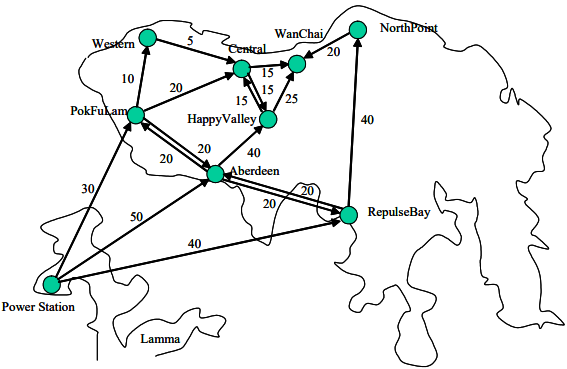
\includegraphics[scale=0.45]{assets/FluxoMaximo/Screenshot_1.png}    
\end{center}

\end{frame}

\begin{frame}{Apresentação do problema}

\begin{outeritemize}
    \item Empresa produtora de carrinhos de golfe
    \item Carrinhos enviados de Detroit para São Francisco de trem, em compartimentos de carga limitada
    \item Máximo de compartimentos que podem ser enviados diariamente
\end{outeritemize}

\begin{center}
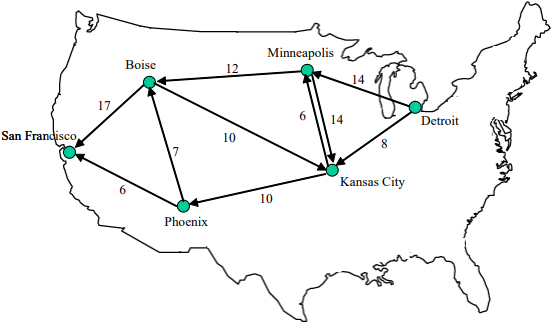
\includegraphics[scale=0.45]{assets/FluxoMaximo/Screenshot_2.png}    
\end{center}

\end{frame}

\begin{frame}{Modelagem do problema}{Definição dos parâmetros e variáveis}

Grafo $G$ ($\mathcal{V}$,$\mathcal{E}$)
\begin{outeritemize}
    \item Conjunto de nós $\mathcal{V}$
    \item Conjunto das arestas $\mathcal{E}$
    \item Limite (inferior/superior) das arestas $(l_{ij}, L_{ij})$
    \item Nó de origem $s$
    \item Nó de destino $t$
\end{outeritemize}

Variáveis
\begin{outeritemize}
    \item Quantidade de fluxo \textbf{do nó $i$ para o nó $j$}
    \item $x_{ij}\geq 0\quad\forall (i,j)\in \mathbb{R}$
\end{outeritemize}

\end{frame}

\begin{frame}{Modelagem do problema}{Restrições}

Respeito ao limites dos enlaces
\begin{outeritemize}
    \item Limite inferior: $$x_{ij}\geq l_{ij}\qquad\forall(i, j)\in \mathcal{E}$$
    \item Limite superior: $$x_{ij}\leq L_{ij}\qquad\forall(i, j)\in \mathcal{E}$$
\end{outeritemize}

Conservação do fluxo
\begin{outeritemize}
    \item Fluxo que entra em $i$ - fluxo que sai de $i = 0$ (exceto para os nós de origem e destino $s$ e $t$)
    $$\sum_{j|(j,i)\in \mathcal{E}}x_{ji}-\sum_{j|(i,j)\in \mathcal{E}}x_{ij}=0\qquad \forall i\in \mathcal{V}\backslash \{s,t\}$$
\end{outeritemize}

\end{frame}

\begin{frame}{Modelagem do problema}{Função objetivo}

Objetivo
\begin{outeritemize}
    \item Maximizar o fluxo que sai de $s$ (ou o que chega em $t$)
    \item Maximizar $$\max\sum_{j|(s,j)\in \mathcal{E}}x_{sj}$$ ou, alternativamente, maximizar $$\max\sum_{i|(i,t)\in \mathcal{E}}x_{it}$$
\end{outeritemize}

\end{frame}

\begin{frame}{Resultado final}

Maximizar $$\max f(\vec{x}) =  \sum_{j|(s,j)\in \mathcal{E}}x_{sj}$$

sujeito a 
$$x_{ij}\geq l_{ij}\qquad\forall(i, j)\in \mathcal{E}$$
$$x_{ij}\leq L_{ij}\qquad\forall(i, j)\in \mathcal{E}$$ 
$$\sum_{j|(j,i)\in \mathcal{E}}x_{ji}-\sum_{j|(i,j)\in \mathcal{E}}x_{ij}=0\qquad \forall i\in \mathcal{V}\backslash \{s,t\}$$ 
$$x_{ij}\geq 0\qquad x_{ij}\in \mathbb{R}$$

\end{frame}

%Felipe Táparo
\subsection{Roteirização}
\begin{frame}{Introdução}{Problema}

\begin{outeritemize}
    \item Dados
    \begin{itemize}
        \item Localização, quantidade e demanda dos pontos a serem atendidos.
        \item Frota de veículos disponíveis e sua capacidade.
        \item Distância e tempo de viagem entre todos os pares de pontos.
    \end{itemize}
\vspace{0.5cm}
    \item Determina-se
    \begin{itemize}
        \item Quantidade de veículos.
        \item Alocação do papel de cada veículo.
        \item Definição de rotas.
    \end{itemize}
\end{outeritemize}
\end{frame}


\begin{frame}{Problemas de Roteirização}
    \begin{columns} 
    \begin{column}{.5\textwidth}
        \begin{outeritemize}
        \item Roteirização sem restrição
        \begin{itemize}
            \item Encontrar sequência de visitas que minimize o percurso.
        \end{itemize}
        \vspace{0.5cm}
        \item Roteirização com restrição
        \begin{itemize}
            \item Considera restrições de capacidade e tempo.
        \end{itemize}
        \end{outeritemize}
    \end{column}
    \begin{column}{.5\textwidth}
        \begin{center}
        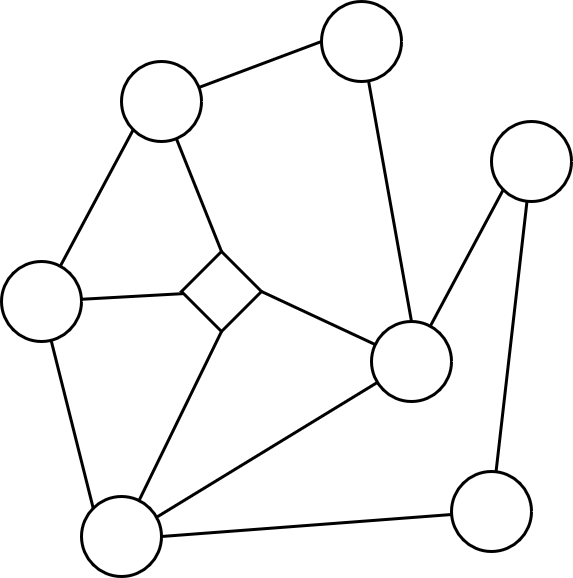
\includegraphics[scale=0.20]{assets/Roteirizacao/R1.png}    
        \end{center}
    \end{column}
    
\end{columns}
\end{frame}

\begin{frame}{Roteirização sem restrição}{Problema do caixeiro viajante}
    \begin{outeritemize}
        \item Encontrar a menor rota para percorrer uma série de nós, retornando ao nó inicial.
        \item Nós deverão ser vizitados apenas uma vez
        \item Exemplo em roteirização: sistema de entregas, correios...

    \end{outeritemize}
\end{frame}

\begin{frame}{Roteirização sem restrição}{Modelagem}
Função Objetivo:
$$
\textrm{min}\sum_{i=1}^{n}\sum_{j \neq i, j=1}^{n} c_{i,j} x_{i,j}
$$
onde
$$
x_{i,j} = \begin{cases}
    1 \textrm{ se o veículo passa por esse caminho} \\
    0 \textrm{ caso contrário}
\end{cases}
$$
$$
c_{i,j} \textrm{ é o custo de ir de i para j}
$$

\end{frame}

\begin{frame}{Roteirização sem restrição}{Modelagem}
Sujeito a

$$
\sum_{i=1}^{n} x_{i,j} = 1, \quad \forall j \in \{1,2,3,...,n\} 
$$
$$
\sum_{j=1}^{n} x_{i,j} = 1, \quad \forall i \in \{1,2,3,...,n\} 
$$

\end{frame}

\begin{frame}{Roteirização sem restrição}{Modelagem - Subrotas}
Modelo não excluí a existência de subrotas!\\
São necessárias restrições adicionais\\
    \begin{center}
        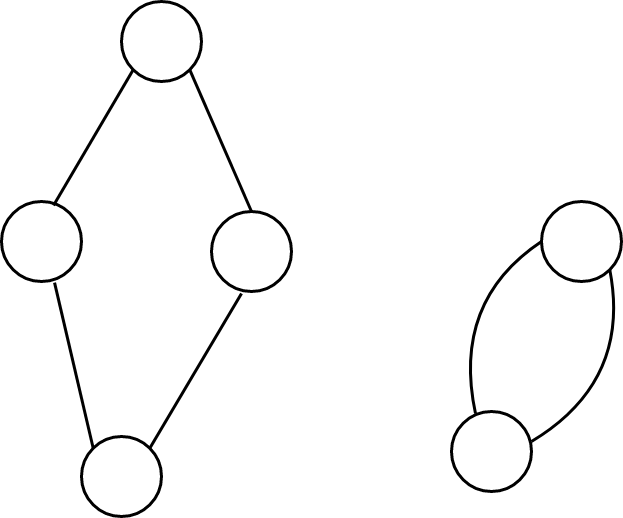
\includegraphics[scale=0.20]{assets/Roteirizacao/sub.png}    
    \end{center}
\end{frame}

\begin{frame}{Roteirização sem restrição}{DFJ}

Dantzig, Fulkerson e Johnson (DFJ):
$$ \sum_{i \in S}\ \sum_{j \neq i, j \in S} x_{i,j} \le |S|-1, \quad \forall S \subsetneq \{1,2,...,n\}, |S|\ge 2$$
\begin{itemize}
    \item Para todo subconjunto $S$ diferente do conjunto completo, o número de arestas deve ser menor ou igual que o número de vértices do subconjunto
\end{itemize}

\end{frame}

\begin{frame}{Roteirização sem restrição}{MTZ}

Modelagem Miller, Trucker Zemlin (MTZ):
$$u_1 = 1,$$
$$2 \le u_i \le n \quad \forall i \in \{2,...,n\},$$
$$u_i - u_j + nx_{i,j}\le n-1 \quad \forall (i,j) \in \{2,...,n\}, i \ne j$$
\begin{itemize}
    \item $u_i$ representa o número de nós vizitados anteriormente
    \item Gera uma nova variável para cada nó
    \item Gera $n+(n-1)+(n-2)$ novas restrições
    \item Conjunto de inequações não tem solução para subrotas
\end{itemize}
\end{frame}

\begin{frame}{Exemplos de heurísticas}
\begin{itemize}
        \item Problema: complexidade cresce exponencialmente
        \item Solução a partir de heurísticas
    \end{itemize}
\begin{columns} 
    \begin{column}{.5\textwidth}
    \begin{center}
    Sem restrição\\
    Vizinho mais próximo
    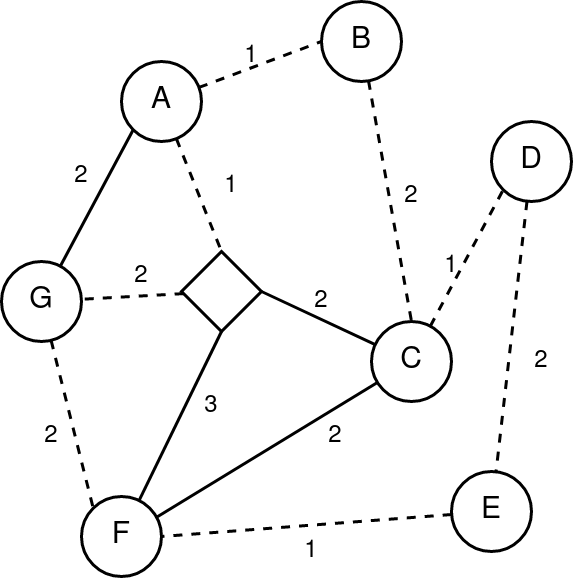
\includegraphics[scale=0.20]{assets/Roteirizacao/vp5.drawio.png}
    \end{center}
    \end{column}
    \begin{column}{.5\textwidth}
    \begin{center}
    Com restrição\\
    Varredura
    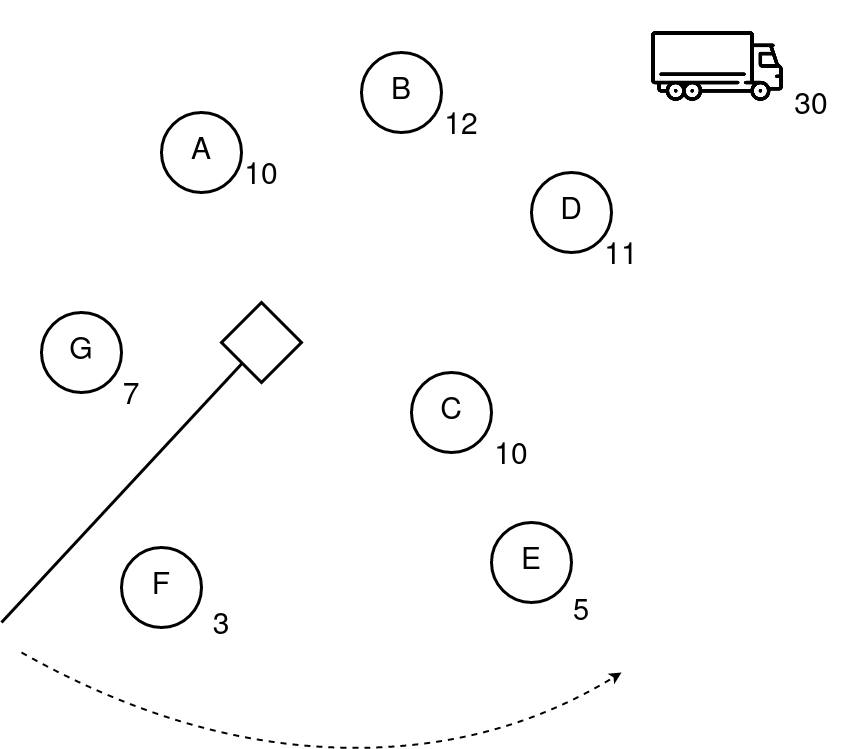
\includegraphics[scale=0.18]{assets/Roteirizacao/Varredura.drawio.png}
    \end{center}
    \end{column}
\end{columns}
    
\end{frame}

%\begin{frame}{Roteirização sem restrição}{Heurística do Vizinho mais próximo}
%    \begin{columns} 
%    \begin{column}{.5\textwidth}
%        Para cada passo adiciona-se à solução o nó mais próximo ainda não visitado.
%    \end{column}

%    \begin{column}{.5\textwidth}
%        \begin{center}
%        \begin{overprint}
%        \onslide<1>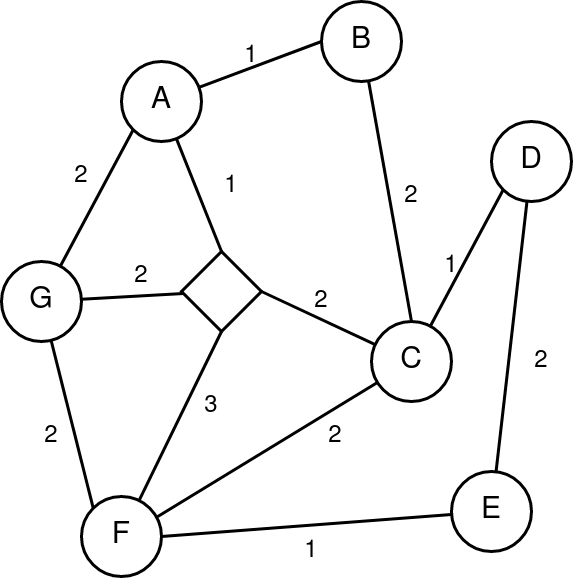
\includegraphics[scale=0.20]{assets/Roteirizacao/vp1.drawio.png}
%        \onslide<2>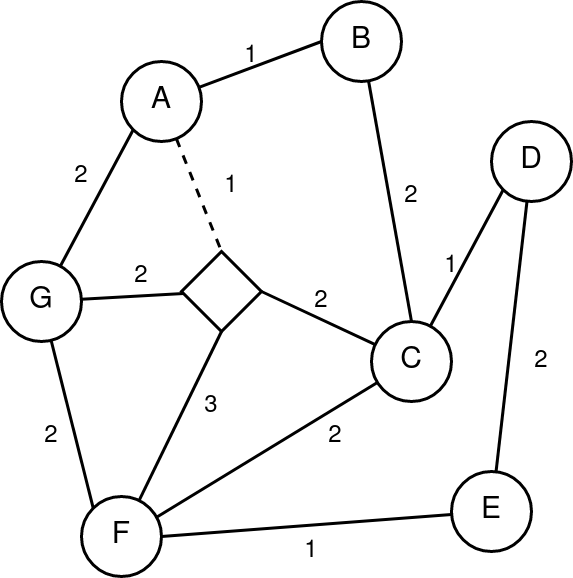
\includegraphics[scale=0.20]{assets/Roteirizacao/vp2.drawio.png}
%        \onslide<3>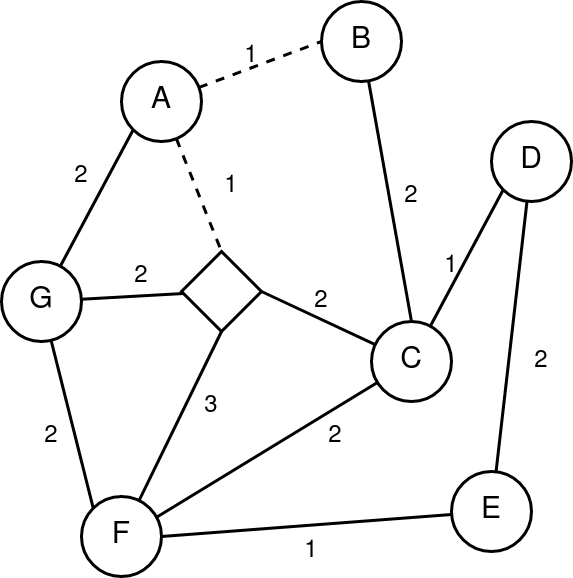
\includegraphics[scale=0.20]{assets/Roteirizacao/vp3.drawio.png}
%        \onslide<4>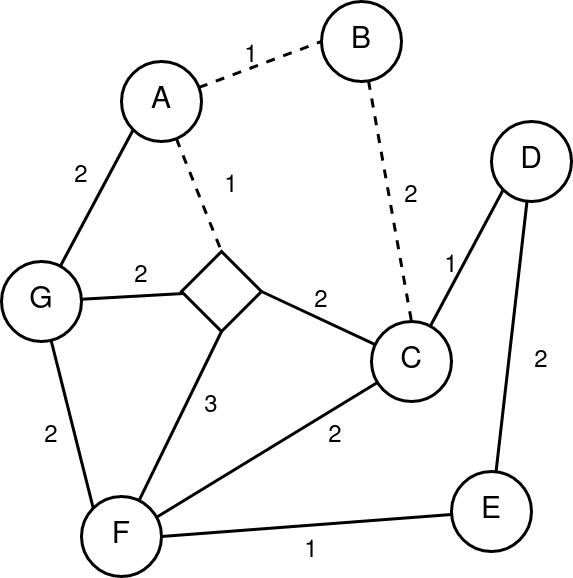
\includegraphics[scale=0.20]{assets/Roteirizacao/vp4.drawio.png}
%        \onslide<5>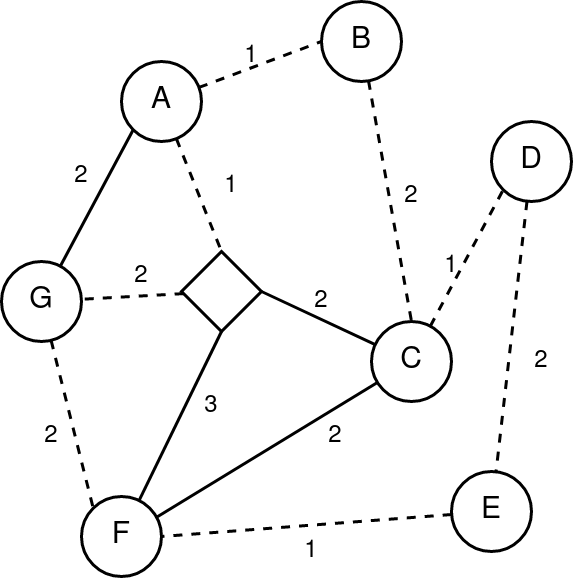
\includegraphics[scale=0.20]{assets/Roteirizacao/vp5.drawio.png}
%        \end{overprint}
%        \end{center}
%    \end{column}
%\end{columns}
%\end{frame}

%\begin{frame}{Roteirização com restrição}
%\begin{outeritemize}
%    \item Preocupa-se com restrições de capacidade e tempo.
%    \item Métodos para resolução
%    \begin{itemize}
%        \item Varredura
%        \item Clarke \& Wright
%    \end{itemize}
%\end{outeritemize}
%\end{frame}

%\begin{frame}{Roteirização com restrição}{Varredura}
%\begin{columns}
%    \begin{column}{.5\textwidth}
%        \begin{itemize}
%            \item Toma-se o ponto de partida como centro.
%            \item Gira um eixo em torno do centro até encontrar um nó.
%            \item Verifica se o nó pode ser incluído no roteiro em formação.
%            \item Caso contrário inicia-se um novo roteiro.
%            \item Para cada roteiro aplica-se um método de otimização de forma a minimizar o percurso.
%        \end{itemize}
%    \end{column}
    

%    \begin{column}{.5\textwidth}
%        \begin{center}
%        \begin{overprint}
%        \onslide<1>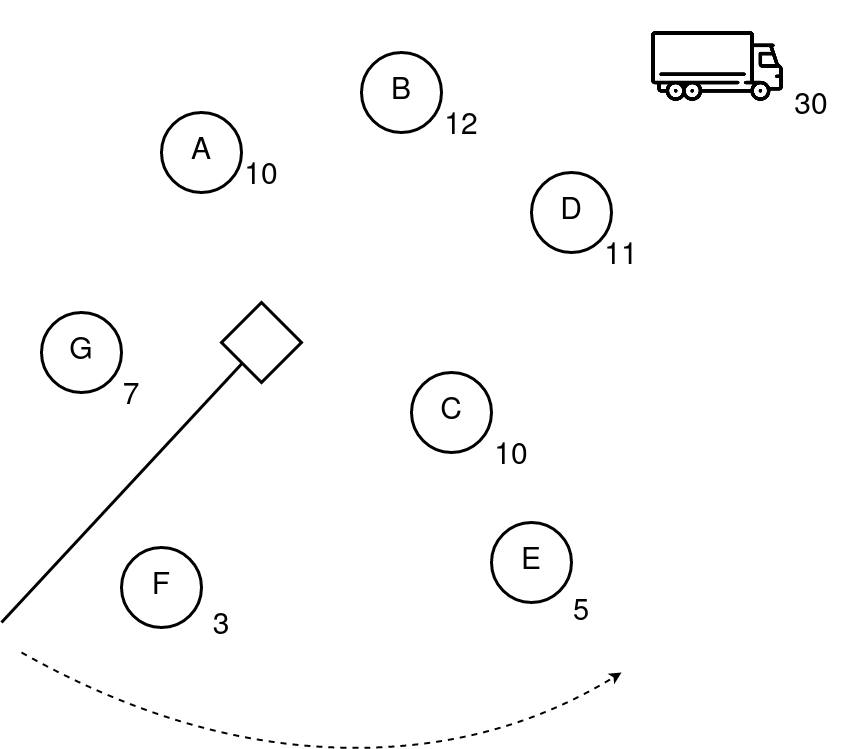
\includegraphics[scale=0.18]{assets/Roteirizacao/Varredura.drawio.png}
%        \onslide<2>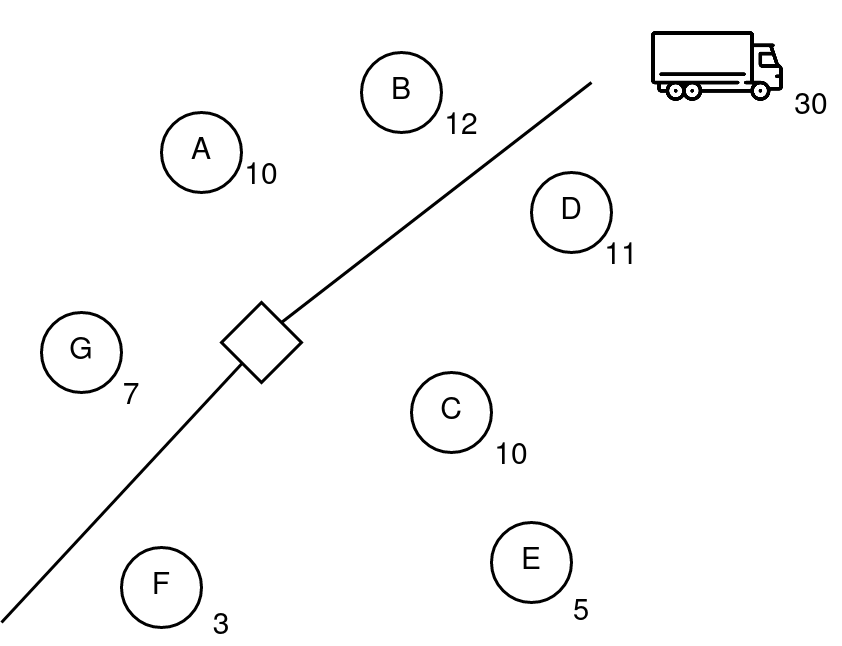
\includegraphics[scale=0.18]{assets/Roteirizacao/Varredura2.png}
%        \onslide<3>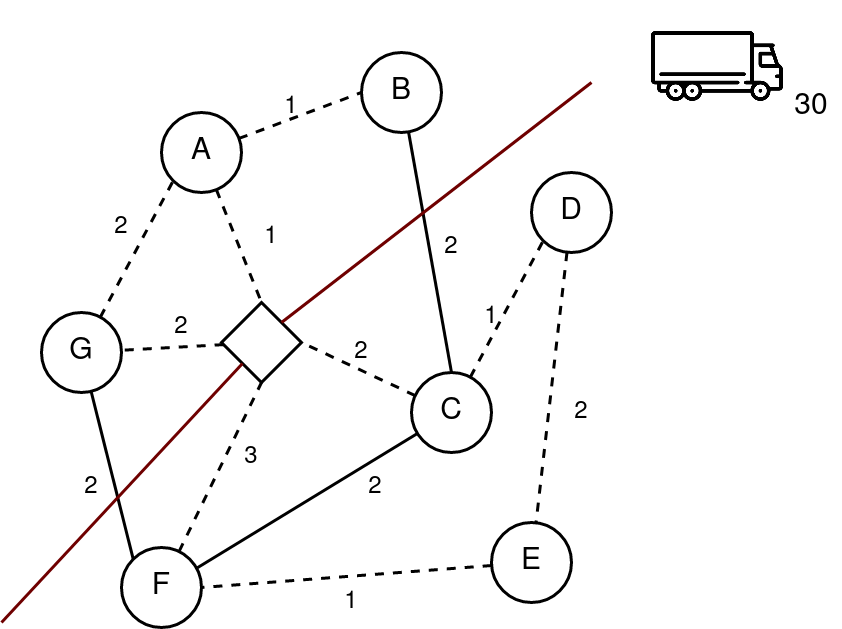
\includegraphics[scale=0.18]{assets/Roteirizacao/Varredura3.png}
%        \end{overprint}
%        \end{center}
%    \end{column}

%\end{columns}
%\end{frame}

% Alan
\section{Métodos de resolução}

\subsection{Introdução e Algoritmos}


\begin{frame}{Como resolver problemas de otimização}
    
    Exitem diferentes tipos de métodos de otimização.
    
    \begin{itemize}
        \item Métodos lineares.
        \item Métodos Não-lineares
    \end{itemize}
\end{frame}

\begin{frame}{Métodos de programação linear}

\vspace{12pt}
Vantagens de modelos lineares:
\begin{itemize}
    \item Simples de resolver.
\end{itemize}

Desvantagens:
\begin{itemize}
    \item A maioria dos problemas de otimização não são lineares.
    \item Modelos lineares normalmente são simplificações dos problemas reais.
\end{itemize}
\end{frame}


\begin{frame}{Métodos não-lineares}
    
    Exemplos de métodos de solução para problemas não lineares:

    \begin{itemize}
        \item Método do gradiente descendente.
        \item Algoritmo genético (evolutivo).
        \item Annealing simulado.
    \end{itemize}
\end{frame}

\begin{frame}{Annealing simulado}
    \begin{itemize}
    \item É um algoritmo probabilístico usado para encontrar o máximo ou mínimo global.
    \item Aplicável em cenários complexos, com muitas variáveis discretas ou contínuas.
    \item Inspirado em um processo físico, que envolve o aquecimento e resfriamento controlado de um material.
    \item Precisa de um modelo que relaciona os parâmetros de decisão com as quantidades a serem minimizadas.
    \end{itemize}
\end{frame}

\begin{frame}{Parâmetros do modelo}
    \begin{itemize}
        \item Estados iniciais (variáveis a serem otimizadas).
        \item Temperatura inicial (relacionado ao passo máximo).
        \item Temperatura mínima (quando parar o algoritmo).
        \item Critério de seleção do novo estado.
        \item Condição de equilíbrio (condição para mudar a temperatura).
    \end{itemize}
\end{frame}

\begin{frame}{Ilustração}
    \begin{figure}
            \centering
            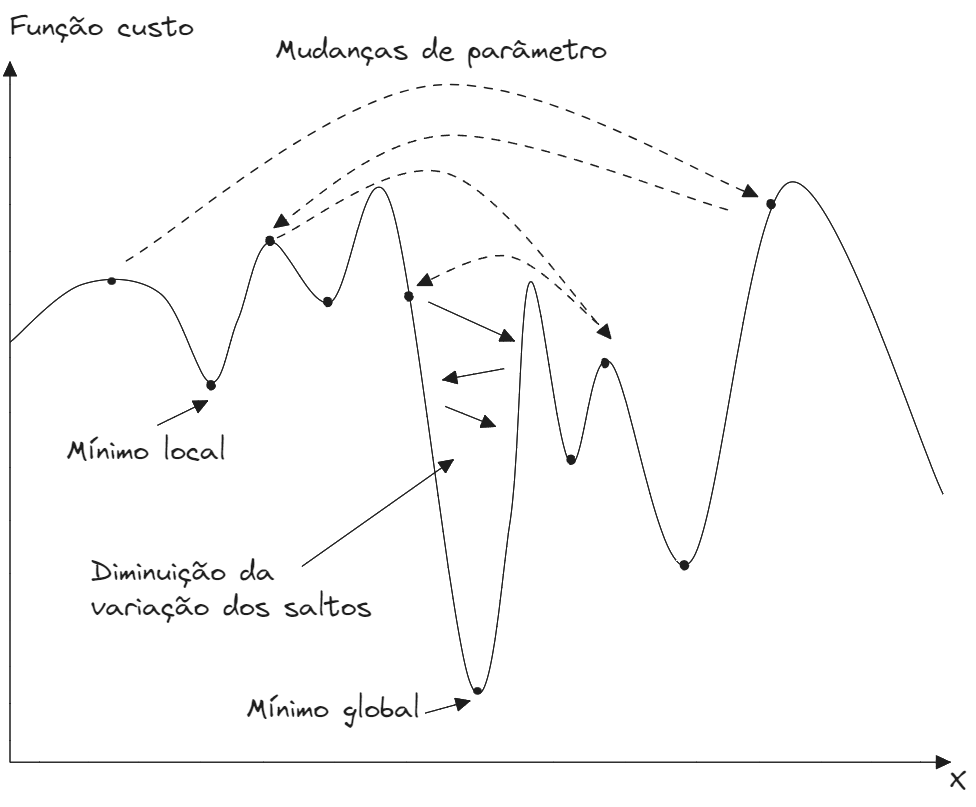
\includegraphics[width = 0.8\textwidth]{assets/Resolucoes/Annealing-Alan.png}
            \label{fig:Annealing}
        \end{figure}
\end{frame}

\begin{frame}{Exemplo de algoritmo}
    \begin{algorithm}[H]
        \begin{algorithmic}[1]
            \STATE $X = X_{init}$ 
            \STATE $T = T_{init}$ 
            \WHILE{$T < T_{min}$}
            \FOR{$i = 0$, $i < N$}
            \STATE $X = X_{old} + f(T, rand)$ 
            \IF{$C(X) < C(X_{old})$ \OR rand  $ < e^{\frac{C(X) - C(X_{old})}{KT}}$} 
            $X_{old} = X$ 
            \ENDIF
            \ENDFOR
            \STATE $T = \alpha T$
            \ENDWHILE
            \RETURN $X_{old}$
        \end{algorithmic}
        \caption{Exemplo de annealing simulado}
        \label{alg:algoritmo}
    \end{algorithm}
\end{frame}

\begin{frame}{Aplicação no problema de roteirização}

    Considere que gostariamos de minimizar a distância total percorrida entre 20 cidades representadas por pontos em um mapa:
    
    \begin{figure}
        \centering
        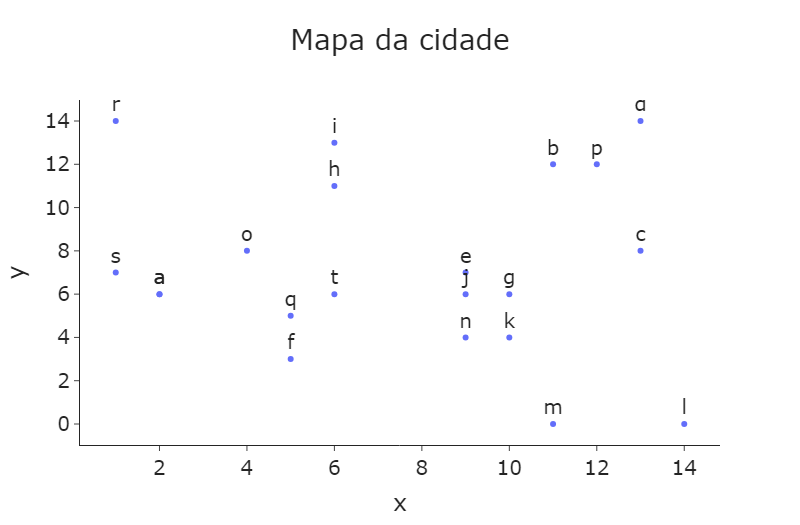
\includegraphics[width = 0.8 \textwidth]{assets/Resolucoes/Cidades.png}
        \label{fig:enter-label}
    \end{figure}
\end{frame}


\begin{frame}{Desempenho do algoritmo}
    \begin{figure}
        \centering
        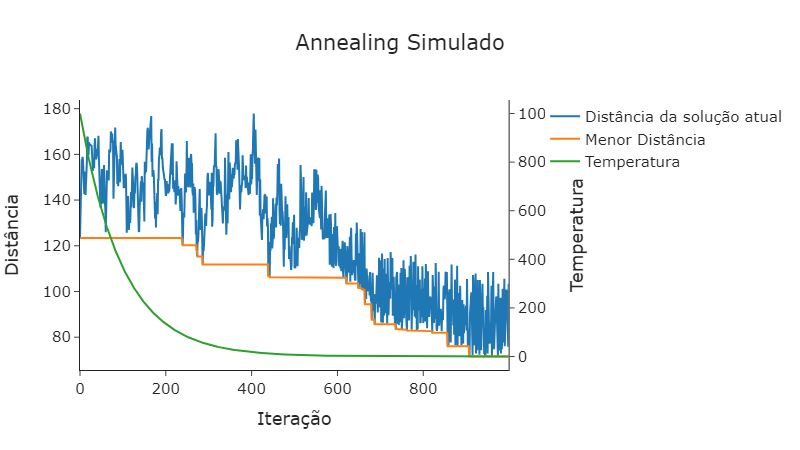
\includegraphics[width = 1 \textwidth]{assets/Resolucoes/evolucao do algoritmo.png}
       \label{fig:enter-label}
    \end{figure}
\end{frame}

\begin{frame}{Aplicação no problema de roteirização - Solução}
     \begin{figure}
        \centering
        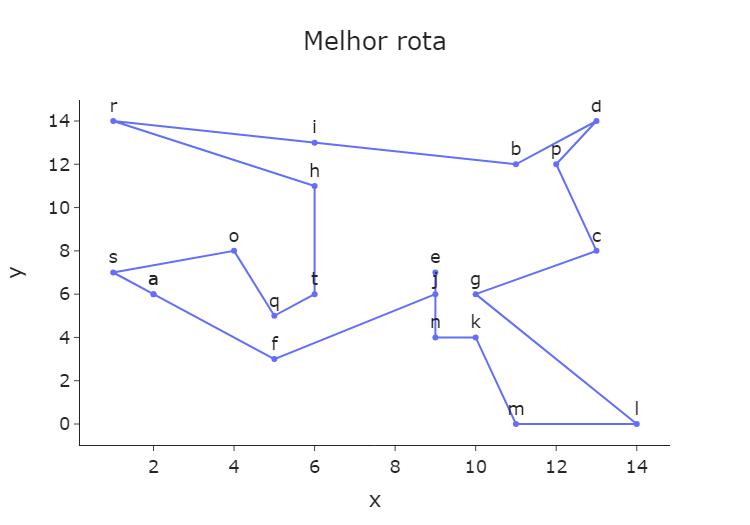
\includegraphics[width = 0.8 \textwidth]{assets/Resolucoes/melhor rota.png}
        \label{fig:enter-label}
    \end{figure}
\end{frame}

\section{Bibliografia}

% Define todas as citações restantes como não citadas
\nocite{*}
\begin{frame}[allowframebreaks]{Referências}
    \printbibliography[category=cited]
\end{frame}

\begin{frame}[allowframebreaks]{Bibliografia}
    \printbibliography[notcategory=cited]
\end{frame}

\end{document}
